\documentclass[12pt]{article}
\usepackage{multicol}
\usepackage{cite}
\usepackage{listings}
\usepackage{tikz}
\usepackage[doublespacing]{setspace}
\usetikzlibrary{positioning}

\lstset{basicstyle=\ttfamily}

\author{Sammy Furr}
\title{Teaching Debugging Collaboratively---Midway Report}
\date{\today}

\begin{document}

\begin{titlepage}
\maketitle
\end{titlepage}

\section{Introduction}

Debugging is invaluable in writing and understanding code, yet it is
rarely formally taught\cite{doi:10.1080/08993400802114581}.  We
typically teach students programming structures, concepts, and
languages, but we leave them to learn the tools they use to code by
themselves.  This approach often works well---the programmer's choice
of editor is \textit{very} personal, students figure out how to
configure an individualized workflow.  Perhaps because debuggers are
tools, they often get lumped into the ``teach yourself'' category.
Unlike editors or reference guides however, effectively using a
debugger requires a set of high-level, platform agnostic, teachable
skills.  Teaching these skills is effective, and translates into
better, faster, debugging and
programming\cite{10.1145/3286960.3286970}\cite{10.1145/3361721.3361724}.\par

The use of a debugger is particularly important in a low-level
programming classes, which is often the first time that students
encounter concepts like assembly instructions and memory addresses.
Debuggers such as GDB offer incredibly powerful tools to step through
and inspect running code.  Sadly, low level debugging tools are often
less than intuitive, and provide little to no means for collaboration.
Powerful tools such as RR exist that enable collaborative ``record and
replay'' debugging\cite{DBLP:journals/corr/OCallahanJFHNP17}, but they
lack tools to visualize address spaces and control flow of programs.
Research shows that visualization of these previously unexplored
spaces aids students taking low-level or systems programming
classes\cite{10.1145/3328778.3366894}.\par

The necessity for accessible, collaborative tools for teaching all
aspects of computer science, not the least debugging, has been
exemplified by the current COVID-19 crisis.  Many students don't have
access to a high powered computer (or even a computer at all) to run
tools that allow for collaboration and replay by capturing the entire
state of a virtual machine\cite{10.1145/2843859.2843867}.  Though the
limitations of interacting with a debugger through a phone or
low-powered laptop seem daunting, I believe they are actually
constraints that can help better shape a visualized, collaborative
approach.\par

For my senior project, I want to develop a front-end interface to RR
that enables collaborative debugging and process visualization on a
variety of non-traditional platforms.

\section{The Value of Teaching Debugging}

Before creating a platform for teaching debugging it's of course
important to make sure that teaching debugging is actually valuable.
There is not a lot research specifically into the efficacy of teaching
debugging for computer science students, despite a recent rise in the
inclusion of debugging in ``computational thinking''
curriculums\cite{10.1145/3361721.3361724}.  These curriculums attempt
to teach skills in computer science classes that are useful in other
subject areas: the UK's computer science curriculum considers
debugging an essential ``transferable skill''\cite{10.1145/2602484}.
Though there seems to be confidence that the problem-solving
techniques used in debugging are widely applicable, I am more
interested in whether systematically teaching debugging actually
benefits computer science students.  Michaeli and Romeike conducted a
good, albeit somewhat small, study on the efficacy of teaching a
systematic debugging process to K12 students.  They found that
students who have been taught a specific debugging framework performed
better in debugging tests and were more confident in their own
debugging skills\cite{10.1145/3361721.3361724}.  Their result is
positive evidence towards the efficacy of teaching debugging, though
their research doesn't include college or university students.\par

As Michaeli and Romeike point out, there is a lack of research into
the value of teaching debugging in higher education.  None of the
research they found placed much focus on explicitly teaching
debugging.  Chmiel and Loui studied whether students who were provided
with debugging tools and frameworks performed better on tests or spent
less time on assignments than those who were
not\cite{10.1145/971300.971310}.  They weren't able to find conclusive
evidence towards better performance on tests or assignments, though
they did find that students in the treatment group felt more confident
in their debugging abilities.  Unfortunately their study didn't
involve extended explicit teaching of debugging---use of the tools was
voluntary, and variations in the students' individual abilities made
the data difficult to evaluate.\par

Despite the lack of higher education-specific research, I feel that
the value of teaching debugging has still been demonstrated.  The
research discussed all finds that K12 and college students alike
commonly resort to sporadic debugging techniques when beginning to
learn.  Given this, I see no reason why the conclusive and positive
research toward the benefit of explicitly teaching debugging to K12
students should not apply to their collegiate counterparts.\par

Research into how to best teach debugging is also self-admittedly
sparse.  Chan et al. allow that ``in general research on how to
improve debugging is sporadic''---an observation that leads them to
research a framework to reduce the complexity of teaching
debugging\cite{10.1145/3286960.3286970}.  To organize their framework,
they split debugging knowledge into 5 categories: Domain, System,
Procedural, Strategic, and Experiential.  They then review different
debugging tools and teaching aids---from those that involve writing
code to games---and map tools to the knowledge areas they seek to
address.  After an evaluation of a host of different tools, they claim
to find a few significant faults in current debugging teaching
platforms.  The two of which I seek to address follow:

\begin{enumerate}
\item A lack of back-tracing ability/coverage.
\item A lack of tools addressing system knowledge (an understanding of
  the program to be debugged).
\end{enumerate}

Basing my collaborative debugging platform on RR solves the problem of
back-tracing ability and coverage.  RR is a ``time traveling''
addition to GDB, that allows for unlimited recording and replaying
code execution deterministically, both backwards and
forwards\cite{DBLP:journals/corr/OCallahanJFHNP17}.  By integrating
the debugger with tools to visualize the execution and code space in
an accessible way, I hope to address the issue of system knowledge.
Though the system knowledge gained may be primarily applicable to low
level programming, skills such as visualizing code execution and
memory space are applicable to all types of coding.  These solutions
are discussed in depth in the following sections.

\section{Collaborative Debugger}

% \subsection{Overview}

\subsection{Preexisting Debugging Tools}

\paragraph{Overview of RR}

Time traveling debugging---stepping backwards and forwards through a
program's execution---is supported naively by GDB through the use of
commands such as \lstinline{reverse-continue} and
\lstinline{reverse-stepi}.\cite{gdbman} What RR brings to the table is
the ability to deterministically record and replay the execution of
even very complex programs.  This allows single users to capture and
debug events that may not happen every time a program runs and revisit
debugging later.  Essentially for my planned collaborative debugger,
execution can be replayed and debugged even \textit{on a different
  computer} than the computer that recorded the original execution.
In comparison to solutions like PANDA\cite{10.1145/2843859.2843867}
that rely on capturing the entire state of of a virtual machine to
replay execution, RR records and replays faster, produces far smaller
files, and doesn't force execution inside of a
VM.\cite{DBLP:journals/corr/OCallahanJFHNP17}

\paragraph{Limitations of RR}

RR comes with two major limitations: it is only compatible with the
Linux kernel, and it's deterministic recording and replay relies on a
feature that is only found on modern \textit{Intel} x86 CPUs.  For my
purposes the first limitation is fairly irrelevant---I expect students
to be connecting to a central server in order to execute and replay
code, and most systems classes are taught in Linux.  The second
limitation poses more of a problem for instruction.  Because recording
and replay is limited to x86 CPUs, classes cannot use a debugger based
on RR to teach ARM assembly, which is becoming increasingly popular.
Though this isn't a limitation that solutions like the aforementioned
full-VM recorder PANDA face, RR still maintains the advantage of being
a debugger first and foremost.  Students can learn RR, GDB, and
debugging techniques simultaneously.  Platforms that require entire VM
replay come with far greater performance and instructional overhead.
Because of RR's ease of use and tight integration with GDB, I feel it
is the best choice of platform to base a collaborative debugger on.

\subsection{User Facing Tools}

There are many existing tools to visualize parts of the process space
during execution, such as Python Tutor's C Tutor\cite{pythontutor}.
Likewise, there are excellent platforms like Matt Godbolt's Compiler
Explorer\cite{godbolt} that allow students to easily see the mapping
of C code to assembly.  Unfortunately there are no student friendly
tools such as these that integrate fully with GDB.  There are plugins
that enhance the features of GDB to offer some further visualization,
like GEF\cite{gef}, but these are typically designed with experts in
mind.  While I feel that it is essential for students to learn
real-world tools like GDB, research shows that visualization tools
designed with teaching in mind significantly increase students'
understanding\cite{10.1145/3328778.3366894}.  I want to marry the
teaching-oriented interface of tools like C Tutor and the Compiler
Explorer with the real-world power of GDB and RR.

% \subsection{Mid Level}

\section{Next Steps}

Further research is needed before I start on the user-facing part of
the collaborative debugger.  I feel that it's important to pick and
design visualization tools based on research into what works most
effectively for students.  I also want the visualization tools to be
as general as possible.  Though I plan to use them to visualize x86
programs running in RR, tools like those to visualize registers could
easily be written more generally, allowing them to represent ARM or
MIPS registers.  In order to make the debugger as flexible as possible
I plan on splitting the package into three parts:

\begin{figure}[h]
  \centering
  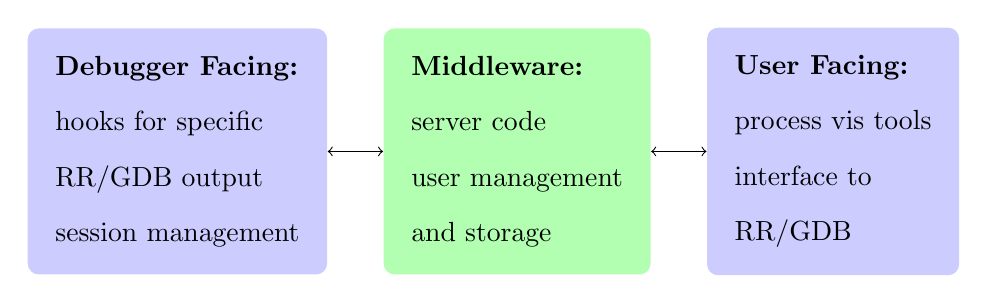
\begin{tikzpicture}
    [node distance = 2em, auto, every node/.style={align=left,
      rectangle, minimum size=2em, rounded corners, fill=blue!20, inner
      sep=1em}, ml/.style = {fill=green!30}]

    \node (ll) 
    {\textbf{Debugger Facing:}\\
      hooks for specific\\
      RR/GDB output\\
      session management
    };
    \node (ml) [ml, right =of ll]
    {\textbf{Middleware:}\\
      server code\\
      user management\\
      and storage
    };
    \node (hl) [right =of ml]
    {\textbf{User Facing:}\\
      process vis tools\\
      interface to\\
      RR/GDB
    };
    \draw[<->] (ll) -- (ml);
    \draw[<->] (ml) -- (hl);
  \end{tikzpicture}
  \caption{\textbf{Blue:} RR specific software. \textbf{Green:} general collaborative
    debugging management}
\end{figure}

I'm not planning to directly extend RR or GDB to add collaborative
debugging features.  Instead, I plan to write code that will hook into
specific RR/GDB outputs and manage a single RR/GDB session.  This code
will interface with server code that manages multiple users and
coordinates collaborative debugging.  The server will pass on commands
to user facing visualization tools, which will translate output from
the debugger to visualizations and provide an interface to RR/GDB.
Segmenting the code in this way allows the addition of different
debugger backends or different front-end vis tools without changing
the code that handles collaboration.  This makes the debugger
extensible as methods and tools evolve.\par

I plan to continue research and begin working on the software over the
summer.  By the beginning of the Fall semester I hope to have made
significant progress on the interface for a single user to RR/GDB.

\pagebreak
\bibliographystyle{acm}
\bibliography{sprojbib}{}
\end{document}
